\subsubsection{Capacitor Plugins}

Plugins sind ein wichtiger Bestandteil von Capacitor.
Sie ermöglichen es, native Funktionen in Capacitor Anwendungen zu integrieren.
Plugins können für Android und iOS implementiert werden.
Mithilfe der Capacitor"=Community Electron Platform können Plugins für Electron implementiert werden, wodurch sie auch unter Windows, Linux und macOS funktionieren.
\cite{capacitor:docs, capacitor-electron}

Beispielsweise ermöglicht das Capacitor Storage Plugin, auf Daten des Geräts zuzugreifen und diese zu speichern.
Mit dem Capacitor Network Plugin können Netzwerkverbindungen geöffnet und Daten übertragen werden.
\cite{capacitor:plugins}

Capacitor bietet eine Vielzahl solcher Plugins offiziell an.
Darüber hinaus hat die Community eine Reihe von Capacitor Plugins entwickelt, die die Funktionalität von Capacitor Anwendungen erweitern können.
Um die Erstellung neuer Plugins zu vereinfachen, bietet Capacitor einen Plugin Generator an.
Dieser generiert alle erforderlichen Dateien, die für den Einstieg benötigt werden.
\cite{capacitor:docs}

\newpage

\paragraph{Funktionsweise von Plugins}

Eine der Philosophien hinter Capacitor Plugins ist, dass sie einen relativ kleinen Umfang aufweisen sollten.
Dadurch werden unnötige Aufblähungen von Apps vermieden und die Bereitstellung, Zusammenarbeit und Wartung von Apps wird erleichtert.
\cite{capacitor:docs}

Aus diesem Grund bestehen Plugins grundsätzlich aus zwei Teilen:

\begin{enumerate}
    \setlength\itemsep{-0.8em}
    \item \textbf{API Definitionen} 
    \item \textbf{Native Implementierung}
\end{enumerate}

Der erste Teil eines Plugins besteht aus einem TypeScript-Interface, das die Signatur der \acs{api}"=Methoden des Plugins definiert und dokumentiert.
Der zweite Teil implementiert alle deklarierten Methoden auf den entsprechenden Plattformen.
\cite{capacitor:docs}

Damit eine Capacitor Anwendung auf die Methoden des Plugins zugreifen kann, wird das TypeScript"=Interface in der Capacitor Runtime registriert.
Wenn die Anwendung eine Methode des Plugins aufruft, führt die Capacitor Runtime die entsprechende native Implementierung dieser Methode aus.

\begin{figure}[H]
    \centering
    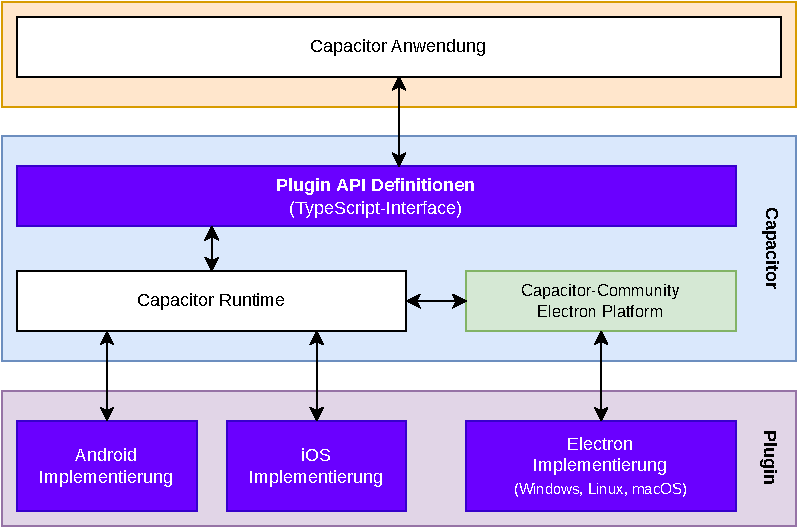
\includegraphics[width=0.8\textwidth]{assets/01_Einführung/01_CapacitorPlugins.pdf}
    \caption{Funktionsweise von Capacitor Plugins}
\end{figure}

\vspace{-1em}

Capacitor bietet für native Implementierungen verschiedene Methodentypen.
Der Void"=Rückgabetyp kann nur einen Fehler zurückgeben.
Der Value"=Rückgabetyp kann auch Daten zurückgeben.
Der Callback"=Typ kann wiederholt Daten an die Capacitor-Anwendung zurückgeben.
\cite{capacitor:docs}

Darüber hinaus können in dem TypeScript"=Interface auch Konfigurationen für das Plugin definiert werden.
Anwender des Plugins können Konfigurationen einfach über die Capacitor Konfigurationsdatei vornehmen.
Im Plugin werden diese Konfigurationen dann über eine Methode der Capacitor Runtime ausgelesen.
\cite{capacitor:docs}
